\documentclass[a4paper,11pt]{kth-mag}
\usepackage[T1]{fontenc}
\usepackage{textcomp}
\usepackage{lmodern}
\usepackage{datetime}
\usepackage[utf8]{inputenc}
\usepackage[swedish,english]{babel}
\usepackage{modifications}
\usepackage{graphicx}
\usepackage{subcaption}
\usepackage{url}
\selectlanguage{swedish}
\title{Benchmarking Human Solving Methods for
           Rubik's cube}

\subtitle{Duis autem vel eum iruire dolor in hendrerit in
          vulputate velit esse molestie consequat, vel illum
          dolore eu feugiat null}

\author{Andreas Nilsson  anil9@kth.se\\Anton Spång  aspang@kth.se}
\date{\today}

\blurb{DD143X - Bachelor Thesis\\Supervisor: Michael Schliephake\\Examiner: Örjan Ekeberg}
\trita{TRITA xxx yyyy-nn}
\begin{document}
\frontmatter
\pagestyle{empty}
\removepagenumbers
\maketitle
\selectlanguage{english}
\begin{abstract}
  This is a skeleton for KTH theses. More documentation
  regarding the KTH thesis class file can be found in
  the package documentation.


\end{abstract}
\clearpage
\begin{foreignabstract}{swedish}
  Denna fil ger ett avhandlingsskelett.
  Mer information om \LaTeX-mallen finns i
  dokumentationen till paketet.
\end{foreignabstract}

\clearpage
\tableofcontents*
\mainmatter
\pagestyle{newchap}
\chapter{Introduction}
\begin{figure}
	\centering
	\begin{subfigure}[b]{0.3\textwidth}
		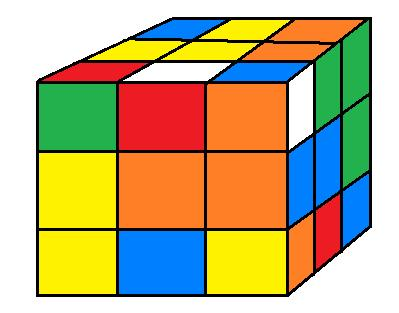
\includegraphics[width=\textwidth]{figs/scramble.jpg}
		\caption{Scrambled cube}
		\label{fig_1}
	\end{subfigure}
	\begin{subfigure}[b]{0.3\textwidth}
		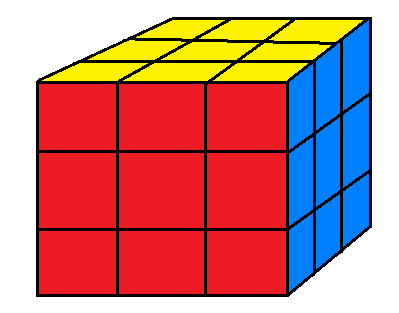
\includegraphics[width=\textwidth]{figs/DONE.png}
		\caption{Solved cube}
		\label{fig_2}
	\end{subfigure}
	\caption{}
\end{figure}
The Rubik’s cube is an 3-D combination puzzle, where each side of the cube is covered with nine squares in six possible colours: white, red, blue, orange, green and yellow.\\
You start with a scrambled cube, meaning that the colored miniature cubes (cubies) are randomly positioned by using random operations on the cube ( fig \ref{fig_1}) . \\
The goal is to obtain the unique solution where each side of the cube are covered with only one colour per side (fig \ref{fig_2}). 
Different methods have been developed with series of notation to solve subproblems one at the time to reach the unique solution. The general idea which many methods are based on is to solve it one layer at the time.\\
If you were to randomly rotate the faces in an attempt to solve the cube, there is almost zero chance of achieving the solved state in your lifetime because of all the possible permutations of the cube. There are $4.3 * 10^(19)$ (or 43 quintillion) \cite{Faculty} different states. Assuming you get to a unique state every second it would take more than 130 billion years to test 10\% of the cubes possible states [appendix A].\\
There are two major ways to compete in solving the Rubik’s cube: the least amount of moves and solving the cube as fast as possible (speedcubing).
The cube was invented by the professor of architecture Ernő Rubik as a teaching tool to help his student understand 3D objects. It was not until he scrambled his new cube and tried to restore it, that he realize that his creation was a puzzle.\\ 
The cube was originally called magic cube and was licensed to be sold by the american toy company Ideal Toy Company in 1980. \cite{Rubiks}.


\section{Problem Definition}
This thesis will explore two commonly known beginner methods for human solving of rubik’s cubes. Both based on the idea to solve the cube one layer at the time which is the easiest way for the human mind to solve this kind of problem \cite{Lar5}. We will evaluate both methods operation variance, number of operations and time to solve,  to find the most time-efficient and move-efficient of them both.\\

During the literature study there was no such comparison of solving-methods for 3x3x3 cube found. The information found about solving-methods for 3x3x3 cubes was tutorials of how to use them..

\section{Problem Statement}
Which of the beginner algorithms would be more effective for speedcubing?\\
Which of the beginner algorithms solves the cube with the least amount of moves?\\
Which beginner algorithm is easiest to learn and execute to someone inexperienced with the cube?\\
\section{Purpose}
The purpose is to test two methods for solving rubik’s cube to find out which uses the least amount of moves and if the same method is less time-consuming than the other. The inexperienced user will find this as a guideline as to which algorithm to start his/her journey towards solving the Rubik’s cube.
\section{Structure}
The second section will introduce the reader to concepts necessary to understand the algorithms implemented and benchmarked. The third section will explain the methods used in this thesis. The fourth sections will explain the implementations made in detail and the difficulties.\\
The fifth section will be for presenting the results and the sixth section for discussion regarding the results. After that will there be a conclusions section that completes the circle of the thesis, answering the problem statements. Lastly the references used to this thesis will be listed followed by appendix containing computations and graphs.   


\chapter{Background}
Providing the reader with information of how the cube works and operations that you can perform on it as well as the algorithms that are in focus for this thesis.
\section{Competitions}
There are two types of competitions regarding the cube.
\subsection{Speedcubing}
When competing in an official event regulated by the World Cube Association (WCA), the competitor has at maximum 15 seconds of inspection time of the cube before the solve begins.\cite{WCA2} The time stops when the competitor have reached the unique solution. 
\subsection{Fewest moves}
The competitors have 60 minutes without any inspection time and the competitor should also be able to hand in a written solution with the notations used in the correct format \cite{WCA2}.
\section{Rubik's Cube}
Explanation of how the cube is constructed and the different notations for the operations.
\subsection{Description}
The cube consists of 26 cubies with three,two or one visible sides depending on the type of cubie. There is one core piece consisting of three axes which holds the center pieces together \cite{MadeHow}. 
  The corner and edge pieces (fig \ref{fig_3})  are the cubies that are movable to different edge and corner positions, the center pieces (fig \ref{fig_3}) can only be moved according to the axis.  
\subsection{Notation}
The notation describes the different move operations on the cube. This thesis uses the notation used by WCA. Explained below:\\
Clockwise 90 degrees:\\
F - Front face\\
B - Back face\\
R - Right face\\
L - Left face\\
U - Upper face\\
D - Bottom face\\
To denote the anti-clockwise 90 degrees rotation just put a single citation mark (‘) after the letter. For example F’ - move front face anti-clockwise 90 degrees.\cite{WCA1}
To denote clockwise 180 degrees rotation just put (2) after the letters described above. 
\begin{figure}[b]
	\centering
	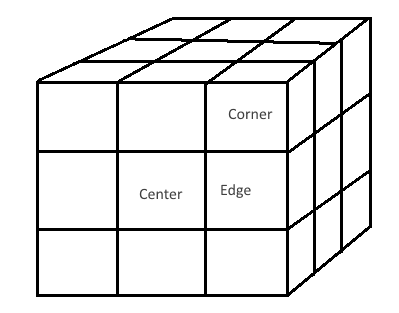
\includegraphics[width= 0.5\textwidth]{figs/representation.png}
	\caption{Cubie types}
	\label{fig_3}
\end{figure}
\section{Algorithms}
The algorithms are physically methods for solving the cube by hand but matches the mathematical definition of an algorithm. Unlike many of the “near-optimal solvers” (some of simulates several moves ahead to find the optimal move\cite{Kociemba}), these algorithms can with little effort be taught to humans.
\subsection{Layer-by-layer using daisy method}
\begin{figure}
	\centering
	\begin{subfigure}[!b]{0.3\textwidth}
		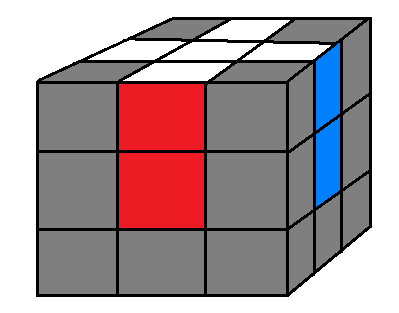
\includegraphics[width=\textwidth]{figs/step1.png}
		\caption{The white cross done}
		\label{fig_4}
	\end{subfigure}
	\begin{subfigure}[!b]{0.3\textwidth}
		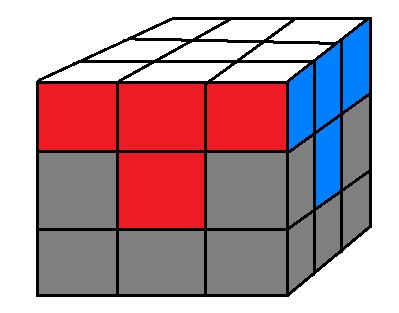
\includegraphics[width=\textwidth]{figs/step2.png}
		\caption{First layer complete}
		\label{fig_5}
	\end{subfigure}
	\caption{}
\end{figure}
The layer-by-layer  (LBL) algorithms divides the cube into layers and makes it possible to solve the subproblems without breaking any pieces already made. 
The daisy method is to solve the white cross by first make a cross with white edges and a yellow center and then turn the white edges, completing the white cross in the bottom \cite{Shellie}.
\subsubsection{1. White cross}
The goal here is to achieve a white cross, so that the white center-piece is aligned with its 4 white edge-pieces in the bottom. For it to be a completed step, the second color of the white edge-pieces must also align with it’s center-piece counterpart as shown in fig \ref{fig_4}. This is done by first making a cross on the top with the yellow center-piece and then flip the edges over to the bottom one at the time using an operation, to make sure the edge-pieces on the vertical sides are aligned with the center-pieces.
\subsubsection{2. White corners}
With the white cross done the next step is to complete the first layer by positioning the white corner-pieces correct between the cross edges (fig \ref{fig_5}). This is achieved with three different operation-combinations depending on the colour positions, all focusing on the upper-front-left corner of the cube.
\subsubsection{3. Middle layer edges}
The next step is to solve the middle layer by moving down a cubie from the middle of the third layer to the correct position on the second layer (fig \ref{fig_6}). 
\subsubsection{4. Yellow cross}
With the second layer complete (fig \ref{fig_7}) it is time to work on the yellow cross. This is achieved by applying one of two operation-combinations or both depending on how many white pieces that are correct positioned (fig \ref{fig_8}).  
\subsubsection{5. Yellow corners}
Positioning the yellow corners by applying different operations to move the edges depending och how many corners that are in position already. 
\subsubsection{6. Last layer permutation}
Now when the corners of the last layer are in position so that the top is all yellow, the only thing left to do is to positioning the pieces of the last layer so they match with the colours of the vertical sides. 
\begin{figure}[h]
	\centering
	\begin{subfigure}[!b]{0.3\textwidth}
		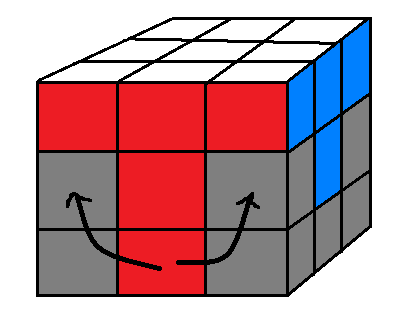
\includegraphics[width=\textwidth]{figs/step32.png}
		\caption{Technique for each side}
		\label{fig_6}
	\end{subfigure}
	\begin{subfigure}[!b]{0.3\textwidth}
		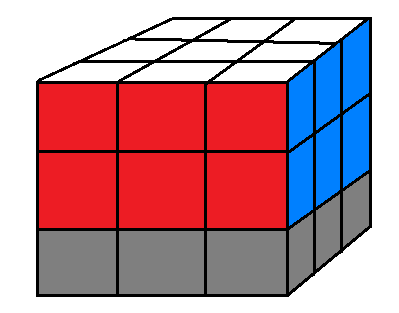
\includegraphics[width=\textwidth]{figs/step31.png}
		\caption{Middle layer complete}
		\label{fig_7}
	\end{subfigure}\caption{}
\end{figure}
\begin{figure}[h]
	\centering
	\begin{subfigure}[!b]{0.3\textwidth}
		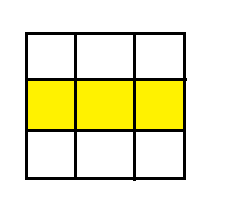
\includegraphics[width=\textwidth]{figs/step41.png}
	\end{subfigure}
	\begin{subfigure}[!b]{0.3\textwidth}
		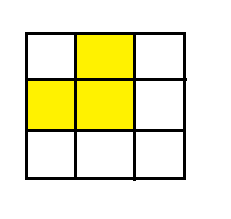
\includegraphics[width=\textwidth]{figs/step42.png}
	\end{subfigure}
	\begin{subfigure}[!b]{0.3\textwidth}
		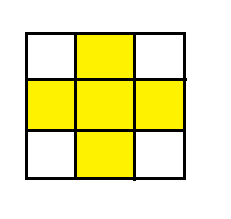
\includegraphics[width=\textwidth]{figs/step43.png}
	\end{subfigure}
	\caption{Different states to achive the yellow cross}
	\label{fig_8}
\end{figure}
\newpage
\subsection{Dedmore algorithm}
\begin{figure}[b]
	\centering
	\begin{subfigure}[!b]{0.3\textwidth}
		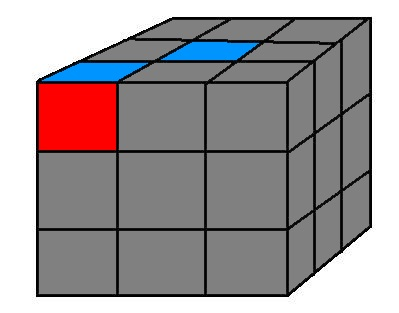
\includegraphics[width=\textwidth]{figs/rubiks-frst-corner.jpg}
		\caption{First corner in position}
		\label{fig_9}
	\end{subfigure}
	\begin{subfigure}[!b]{0.3\textwidth}
		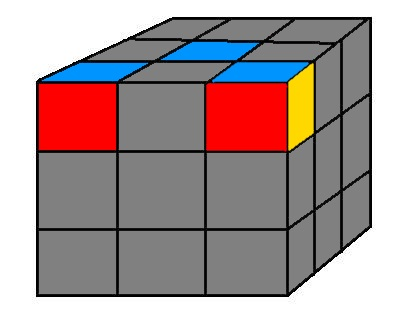
\includegraphics[width=\textwidth]{figs/rubiks-scnd-corner.jpg}
		\caption{Second corner in position}
		\label{fig_10}
	\end{subfigure}
	\begin{subfigure}[!b]{0.3\textwidth}
		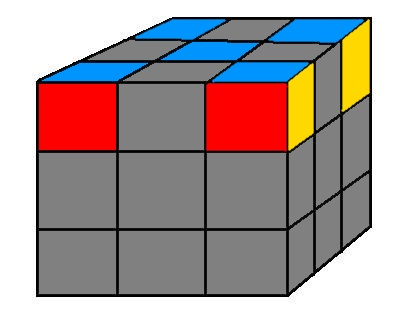
\includegraphics[width=\textwidth]{figs/rubiks-4-corners.jpg}
		\caption{Top edges in position}
		\label{fig_11}
	\end{subfigure}
	\caption{}
\end{figure}

\subsubsection{1. Top corners (the X)}
Start off by finding a starting corner. For example aim to solve the blue top face first. Rotate the cube to obtain the blue side of the corner in top position. Then move the blue center-piece into position without moving your corner. When this is done, rotate the whole cube to obtain the corner in your top left on the front side, as in the fig \ref{fig_9}.\\\\
Next you’ll search for the next corner that should be positioned in the top right front side. Depending on the position on this corner, you will use different operation sequences to get it in position like the fig \ref{fig_10}.\\\\
Simply rotate the cube and continue on. The goal of this step is to form an ‘X’ on the top face as in fig \ref{fig_11}.
\subsubsection{2. Top edges}
The goal of this step is to simply get the edges in place. Get them in place one by one. When this step is finished the cube looks like fig \ref{fig_12}.
\subsubsection{3. Middle layer}
The next step is to solve the middle layer by moving down a cubie from the middle of the third layer to the correct position on the second layer (fig \ref{fig_6}). 

\subsubsection{4. Bottom corners}
Here the cube is turned upside down and the goal here is again to build a (green) X with the corners(fig \ref{fig_13}).
\subsubsection{5. Bottom edges}
In this step, at least one edge is already in the correct place (the color might be switched as in fig \ref{fig_14}). Find that edge and put it on the front side. Then position every other edge correctly by using a series of operations.\\\\
When every edge are correctly positioned, there are 2 possible states left. Each requires a different sequence of operations to solve. The ‘fish’ pattern (fig \ref{fig_15}) and the ‘H’ pattern (fig \ref{fig_16}). Execute the sequence for the pattern and you’ll then have solved the cube.
\begin{figure}[bh]
	\centering
	\begin{subfigure}[!b]{0.3\textwidth}
		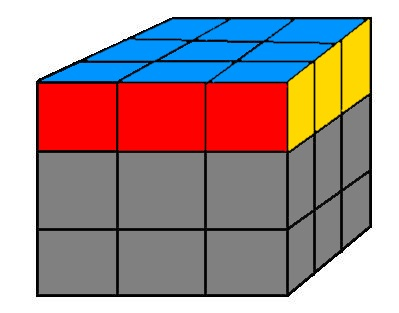
\includegraphics[width=\textwidth]{figs/rubiks-top-edges.jpg}
		\caption{Top edges in position}
		\label{fig_12}
	\end{subfigure}
	\begin{subfigure}[!b]{0.3\textwidth}
		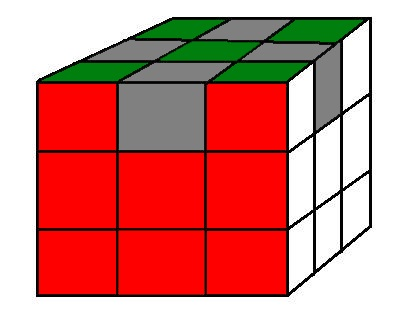
\includegraphics[width=\textwidth]{figs/rubiks-bottom-edges.jpg}
		\caption{The green X}
		\label{fig_13}
	\end{subfigure}
	\begin{subfigure}[!b]{0.3\textwidth}
		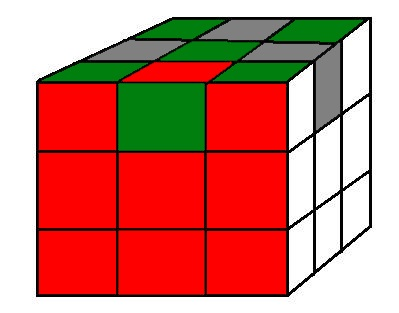
\includegraphics[width=\textwidth]{figs/last-edge-correct.jpg}
		\caption{One edges correctly placed}
		\label{fig_14}
	\end{subfigure}
	\caption{}
\end{figure}
\begin{figure}[bh]
	\centering
	\begin{subfigure}[!b]{0.3\textwidth}
		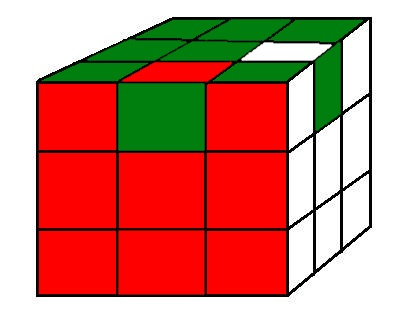
\includegraphics[width=\textwidth]{figs/fish-pattern.jpg}
		\caption{Fish pattern}
		\label{fig_15}
	\end{subfigure}
	\begin{subfigure}[!b]{0.3\textwidth}
		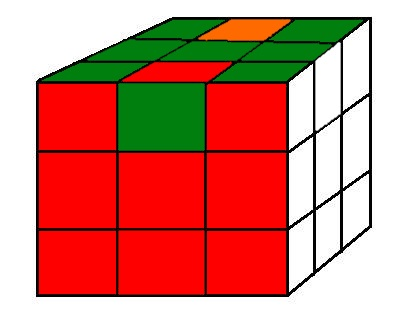
\includegraphics[width=\textwidth]{figs/H-pattern.jpg}
		\caption{H pattern}
		\label{fig_16}
	\end{subfigure}
	\caption{}
\end{figure}

\chapter{Method}

\section{Literature study}
\section{Implementation and data collection}
\section{Analyze and representation}


\chapter{Implementation}
\section{Cube representation}
\section{Algorithms}
\section{Scramble}
\section{Difficulty}

\chapter{Results and Analyze}

\section{Data}
\section{Comparison}

\chapter{Discussion}

\section{Comparison}
\section{Errors}

\chapter{Conclusion}
\cite{MadeHow}
\renewcommand{\bibname}{References}
\bibliographystyle{plain}
\bibliography{references}

\appendix
\addappheadtotoc
\chapter{Calculation of randomly rotate faces}\label{appA}
Our calculations goes here\\

\begin{figure}[ht]
\begin{center}
And here is a figure
\caption{\small{Several statements describing the same resource.}}\label{RDF_4}
\end{center}
\end{figure}

that we refer to here: \ref{RDF_4}
\end{document}
